\documentclass[acmsmall, nonacm]{acmart}

\usepackage[utf8]{inputenc} % allow utf-8 input
\usepackage[T1]{fontenc}    % use 8-bit T1 fonts
\usepackage{hyperref}       % hyperlinks
\usepackage{url}            % simple URL typesetting
\usepackage{booktabs}       % professional-quality tables
\usepackage{amsfonts}       % blackboard math symbols
\usepackage{nicefrac}       % compact symbols for 1/2, etc.
\usepackage{microtype}      % microtypography

\usepackage{amsmath}
%\usepackage{amssymb}
\usepackage{graphicx}
\usepackage{grffile}

\usepackage{longtable}
\usepackage{subcaption}
\usepackage{xcolor}


\title{State description language and PathRL}

% XXX contributors' macros
% gleb
\newcommand{\GG}[1]{\textcolor{red}{[GG: #1]}}
% daniil
\newcommand{\danil}[1]{{\color{red} [#1]}}
% ivan
\newcommand{\attn}[1]{{\color{magenta}{\textbf{#1}}}}


\begin{document}

\maketitle

\section{PathRL algorithm}

\subsection{Definitions}

An MDP is a tuple $(\mathcal{S}, \mathcal{A}, \mathcal{P}, \mathcal{R}, \gamma)$. An observation lies in space $\mathcal{O}$ and is denoted by $O_i$. An inner representation of an observation is denote by $h_i \in \mathcal{H}$. We call a \emph{hash} representation function $
f: \mathcal{O} \rightarrow \mathcal{H}
$. We suppose that the goal agent ``talks'' with the navigation agent via a sequence of messages expressed as points in $\mathcal{H}$.

\begin{figure}
  \centering
  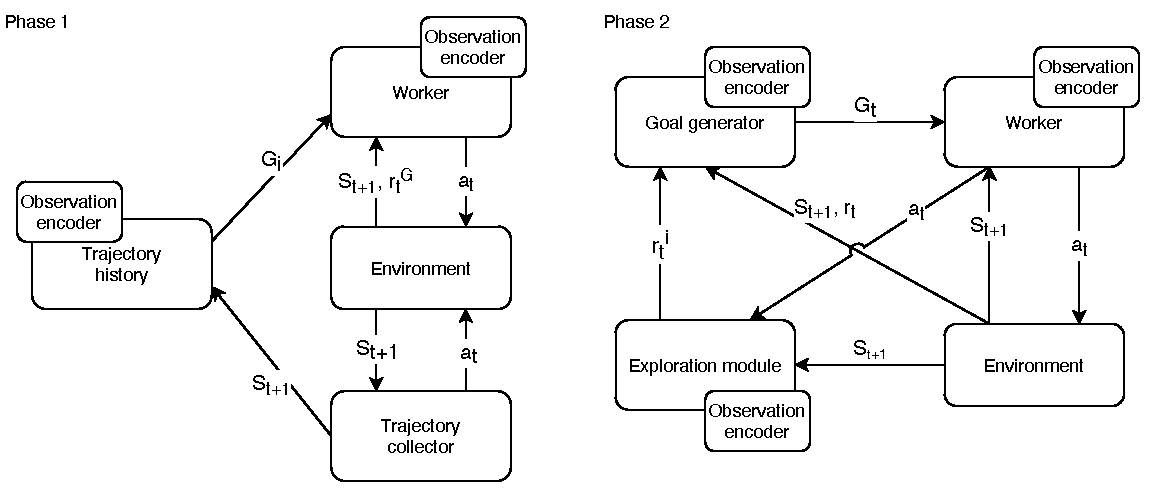
\includegraphics[width=0.9\linewidth]{./assets/diagram.pdf}
  \caption{PathRL alogorithm}
  \label{fig:pathrl}
\end{figure}

\subsection{First phase}


% XXX 1st phase: we just train a navigator using go-explore with HER and curiosity-driven third part explorer
The first phase of training can be described as a two-agent interaction: the encoder agent $E$ learns to produce a description of the task in some restricted inter-agent \emph{language}, and the navigator agent $N$ receives the task description and learns to execute it.
%
The \emph{language} can be similar to a query language wherein the desired state is described in a declarative form of instructions or predicates. The \emph{task} is a pair of queries which specify the initial states and the goals to be reached.
% XXX not just the abstract controllable embedding of target state, but its high level description, generated based on it (rich abstract state embedding). Besdies embedding is likely to be a compressed representation, which makes it unlikely to be a one-to-one mapping on $S$.
%
Both agents are rewarded if the navigator successfully executes the task, i.e. $N$ reaches the a goal set by $E$.
% In current work we consider only the singleton sets of states, hence, the task is defined as a pair of states.
This two-agent game is somewhat similar to the cooperative game proposed by~\citet{Mordatch2018EmergenceOG}.

Formally, the encoder $E$ takes is the desired state $s_g$ and produces its description $E(s_g)$, while the navigator $N$ reacts to this description and the current state $s_t$ by outputting the next action $a_t \sim N(s_t, E(s_g))$. Agent $E$ has no access to the current state $s_t$, which $N$ is in in the environment, and is thus forced to produce some declarative description of the desired state $s_g$, since it cannot communicate the exact sequence of actions $N$ has to perform.
% XXX maybe the target query and a hint vector? as it seems possible that the worker-agent could stray arbitrarily far away from the destination on the embedded state manifold

\subsubsection{Collecting the navigation tasks by exploration}

% the dataset resembles the go-explore-like replay buffer
Training an efficient navigator $N$ requires a diverse dataset of tasks $(s_t, s_g)$, in which a meaningful goal $s_g$ is attainable from the initial state $s_t$. To this end during training \emph{a third agent} randomly traverses the environment using some exploration policy $\mu_e$, thereby generating state-action trajectories that can be mined for feasible training tasks. The policy $\mu_e$ has to meet several requirements: it has to explore the environment reasonably well and the trajectories it produces must be diverse. One of the options is to use curiosity-based exploration \citep{pathak_curiosity-driven_2017,burda_exploration_2019}.
Note, that any state can be selected as initial state $s_t$, if $s_t$ is not the initial state of the environment $s_0$, then, the recorded sequence of previous actions can be executed to reach $s_t$ from $s_0$.

\subsubsection{Navigation reward}
\label{ssub:navigation_reward}

One possible training scheme is to shape the reward so that it encourages moving closer from the current state $s_t$ to the target state $s_g$. The notion of state \emph{proximity} must take into account the fact that states reside on certain latent manifold, must be consistent with respect to environment's randomness, and at the same time focus on controllable and abstract away uncontrollable or irrelevant features of the states. For example, positively rewarding for diminishing Euclidean distance between $s_g$ and $s_t$ fails all these desirable properties.

Specifically, in Random Disco Maze navigation environment, \citep{badia_never_2020}, the pixel-wise distance would hinder the task completion due to irrelevant random color of the labyrinth's walls. In the same environment the initial and goal states that are separated by an adjacent wall, yet unreachable from one another would be considered close states. Finally, in Pac-Man%
\footnote{
    \url{https://en.wikipedia.org/wiki/Pac-Man_(Atari_2600)}
}
the position of the player within the maze is a controllable feature, while the positions of patrolling ghosts are not, yet the distance between states would be sizeable, even if the protagonist has arrived exactly at the specified target position.
%
Similarly with Freeway%
\footnote{
    \url{https://en.wikipedia.org/wiki/Freeway_(video_game)}
}, the player's car is controllable, while the opponents' cars are not, \citep[fig.~1]{choi_contingency-aware_2019}.

% Another scheme is to reward agent from reaching the state that is similar enough to the target state. In this case, the state similarity function is not required to be transitive.

One possibility is to define a proximity score as $
    d(s_a, s_b) 
        := \frac{\phi(s_a)^\top \phi(s_b)}{\|\phi(s_a)\|\|\phi(s_b)\|}
$ -- the cosine similarity between the latent representations of states. The mapping $
    \phi \colon \mathcal{S} \to \mathbb{R}^{d_h}
$ is a learnt state embedding that removes features irrelevant to the navigator's task and effectively flattens the state manifold. The embedding $\phi$, that drops uncontrollable features can be trained in self-supervised manner on the inverse dynamics task. i.e. inferring the action taken between consecutive states, \citep{choi_contingency-aware_2019,badia_never_2020}.

% In this case the function $d(s_a, s_b)$ that estimates the similarity between states is required. The state similarity function should also be transitive i. e. if $d(s_a, s_b) > d(s_a, s_c)$ then $d(s_b, s_c) > d(s_a, s_c)$.
% XXX transitivity is $a \to b$, $b \to c$ implies $a \to c$.
% XXX the property above fails for euclidean distance: take an acute isosceles triangle.

\subsection{Second phase}

The second phase of training of this model is the addition of goal-setting agent $G$ which replaces encoder agent $E$ after training.
% XXX a fourth agent? Wasn't the encoder agent also the goal-setter in the beginning of this section?
% We should emphasize that our methodological contrib is the two-phased training (have to verify this)
%
This goal-setter receives only the current state and produces the set of predicates $e_g = G(s_t)$ that lead to potentially high rewards, i.e. $G$ learns to generate the set of predicates that describe high-reward states. During this phase actions are produced by pre-trained navigator $a_t = N(s_t, G(s_t))$ with frozen parameters, yet differentiable w.r.t. the goal-state embedding. This forces the goal agent $G$ to reproduce and communicate in the same description ``language'' as the encoder agent. This goal-setter is also penalized for the non-reachable goals which worker is failed to achieve.

\subsubsection{Reward scheme}

The goal-setter $G$ is trained with four rewards: the extrinsic reward, i.e. true reward of the environment; the intrinsic curiosity reward for active exploration; and non-reachable goal penalty, received if the worker is not achieved the generated goal for the desired number of steps; short goals penalty, which discourages the goal-setter for setting too close goals for the worker.

In this scheme $G$ is encouraged to propose queries for states of two kinds: \emph{explotable} states with high extrinsic reward, and \emph{explorable}, unknown ``terrritory'' states high curiosity potential.
%
The combination of curiosity reward scheme and navigator agent have some parallels with Go-explore algorithm~\citep{ecoffet_first_2021}, where the navigation is done via virtual environment resets.

\subsubsection{Additional training for the worker}

The worker can be additionally trained during the second phase. During the worker training, the worker weights are unfrozen. The worker is trained on the intrinsic rewards of reaching the generated goals. The goal-setter receives only exploration reward during the worker training.

\subsection{World state representations}

The most promising possibility, especially in the context of the desiderata outlined in sec.~\ref{ssub:navigation_reward}, is to use compressed abstracted representations of the environment states in the encoder, the navigator and the goal-setting agents. The state embeddings can be produced by a world model pre-trained by the next state prediction task, \citep{ha_recurrent_2018}, or by an inverse dynamics model, \citep{badia_never_2020}.

\subsection{Motivation}

% XXX oof, i will reword this later.
The proposed scheme should be effective in sparse extrinsic reward settings: the low-level basic interaction in the environment, when trained to solve the environment on its own, would experience the detrimental effects of reward sparsity most acutely. However, if instead we train a low level agent on state-navigation tasks, motivating it for achieving the goals (a sort of synthetic intrinsic reward, but not curiosity-based), and delegate the solution of the environment itself to an abstract planning agent, which collects extrinsic rewards, we could effectively significantly reduce the planer's reward sparsity. If the high-level agent uses relatively small set of high-level actions (goals) then the number of possible trajectories to explore is drastically reduced: the trajectories of 10 steps of high-level actions will be used instead of trajectories of 100 steps of the low-level actions.

By splitting in two phases we are able to learn efficient reliable navigation skills using synthetic navigation tasks, 
without any extrinsic reward.
%
The proposed two-phase scheme should be effective for the multi-task learning setting in the same environment: a well trained and capable navigator model, even though trained for one specific environment and goal state distribution, can be effectively reused across different tasks.

As shown by \citet{ecoffet_first_2021} the exploration of distant states greatly improves the algorithm effectiveness. The availability of navigator agent enables training a goal agent, which is encouraged to explore remote states.
%
% XXX i am afraid this contribution is more of \citet{badia_never_2020,choi_contingency-aware_2019} rather than ours.
In contrast to \citep{ecoffet_first_2021}, though, by using learnt state representations that abstract away irrelevant information, and by decoupling goal-setting from goal-achieving the scheme proposed in this work may be applied to stochastic and multi-task environments as well.
% XXX ``virtual environment resets'' are useful for faster training and more diverse
%  dataset, their crude state discretization ``hack'', however, is not.

\subsection{Interpretable RL}

The proposed PathRL algorithm can be made interpretable by adding state representation decoder, that would transform a goal back to the desired state, associated with that goal. This can be done training state decoder together with state encoder during the first phase of training.

\subsubsection{Discriminator loss for goal-setter}

To force goal-setter to generate goals, that are state representations, additional discriminator loss can be used. Separate discriminator net can be trained to distinguish between the generated goals and state representations and its accuracy can be used as loss to goal-setter similarly to the GAN training scheme.

\subsubsection{Why goal-setter goals can provide interpretation}

Ideally trained goal-setter should output goals that are keypoint states. The keypoint state of the pair of states $s_b$ and $s_e$, is the state, that can should be included to any trajectory between $s_b$ and $s_e$. The keypoint state of some environment is the state with high \emph{betweenness}, i. e. the state that should be included in many possible trajectories for this environment.

\subsection{Semantic observation attributes}

The alternative, and possibly more scaleable and interpretable approach to PathRL is to use the set of facts about the observation instead of its representation. Each fact is defined as a \href{https://en.wikipedia.org/wiki/Semantic_triple}{semantic triple} (subject, predicate and object), where first and third terms are taken form the same fixed-size set of possible tokens A and second term is taken from another fixed-size set of possible tokens B.

On the first phase the attribute \textit{difference} between the current observation some random observation is calculated. A random subset of attributes from that difference is selected and passed to the worker. The worker goal is to reach any state which have the passed set of attributes. On the second phase the task of goal generator is to produce the subset of attributes that would maximize the reward.

Semantic observation attributes can be manually engineered, or possibly mined from the observations.

\subsubsection{Image guessing}

Observation attributes can possibly be mined using approach considered in language emergence papers. In this scenario the image attributes is learned in the unsupervised setting of image guessing game similarly to~\citet{Havrylov2017EmergenceOL}. In~\citet{Havrylov2017EmergenceOL} the image is transformed into the sequence of tokens, in PathRL, the image is transfromed to the set of facts.


\section{Related work}
\label{sec:related_work}

\paragraph{Feudal RL by~\citet{Dayan1992FeudalRL}} % (fold)
\label{par:feudal_rl}

The task is to find a way in the maze. A hierarchy of policies is defined. A policy use blocks of space as atomic movement positions. Each level of hierarchy use exponentially larger blocks comparing to the previous level. A policy selects a desired block to move to as its action and then assigns a task to lower-level policy. Higher-level policy defines reward for the lower-level policy. The reward for lower-level policy is gained if it successfully guides the agent to the block, defined by the higher-level policy.

% paragraph feudal_rl (end)

\paragraph{STRAW by~\citet{Vezhnevets2016StrategicAW}} % (fold)
\label{par:straw}

The network holds two structures in memory: action plan A and commitment plan c. T-th column of A contains probabilities to perform specific action at time t. c is a vector of probabilities to update the current plan at time t. If $g \sim c_{t-1} = 1$ then the network performs plan update. Both A and c are refreshed during update. The network is trained using A3C.

% paragraph straw (end)

\paragraph{Hierarchical Deep Reinforcement Learning by~\citet{Kulkarni2016HierarchicalDR}} % (fold)
\label{par:hierarchical_deep_rl}

The meta-controller learns an approximation of the optimal goal policy $\pi(g|s)$, i. e. it receives state s and select a goal g from the set of all possible current goals G. The meta-controller operates on the slower time-scale than the controller. The meta-controller receives extrinsic reward from the environment.

The controller learns an approximation of the optimal action policy $\pi(a|g,s)$, i. e. it receives state s and goal g and selects an action a. The internal critic provides intrinsic reward for the controller. For example, a critic for a game can check that specific conditions are fulfilled, e. g. an agent reaches the door.

The critic and the set of possible goals G are not learned but are considered available.

% paragraph hierarchical_deep_rl (end)

\paragraph{HIRO by~\citet{Nachum2018DataEfficientHR}} % (fold)
\label{par:hiro}

Ant Gather / Ant Maze / Ant Push / Ant Fall tasks are used. The higher-level policy instructs the lower-level policy via high-level actions, or goals, which it samples anew every c steps. A higher-level policy takes current state and outputs the goal for lower-level policy. The lower-level policy interacts directly with the environment. The goal simply instructs the lower-level policy to reach the specific state. The reward for lower-level policy is provided if the environment yields an observation close to matching the desired goal.

% paragraph hiro (end)

\paragraph{Curiosity-driven learning by~\citet{pathak_curiosity-driven_2017}} % (fold)
\label{par:curiosity_driven_rl}

Intrinsic Curiosity Module (ICM) predict next state $\hat{s}_{t+1}$ from the current state $s_t$ and action $a_t$ povided by policy network. Difference between predicted $\hat{s}_{t+1}$ and true $s_{t+1}$ is the intrinsic reward for the action $a_t$. Sum of reward from ICM and extrinistic reward is used to train policy network. ICM is in fact a world model.

% paragraph curiosity_driven_rl (end)

\paragraph{Random Network Distillation by~\citet{burda_exploration_2019}} % (fold)
\label{par:random_distillation}

Another approach to the curiosity-driven exploration is proposed by \citep{burda_exploration_2019}. Exploration bonus is based on predicting the output of a fixed and randomly initialized neural network on the next state, given the next state itself. The intuition is that predictive models have low error in states similar to the ones they have been trained on. The method shows better than average human performance on Montezuma’s Revenge.

% paragraph random_distillation (end)

\paragraph{Learning to communicate by~\citet{Mordatch2018EmergenceOG}} % (fold)
\label{par:learning_tom_communicate}

Multi-agent game: one agent knows the task and should communicate that task to other agents via broadcast messages. An example of task is to move other agent to the the specific location in the 2D world.

% paragraph learning_tom_communicate (end)

\paragraph{DADS by~\citet{Sharma2020DynamicsAwareUD}} % (fold)
\label{par:dads}

The authors propose an intrinsic reward, which encourages an agent to learn valuable ``skills''. The intrinsic reward is high if the changes in the environment is predictable for the specific 'skill' and, if the changes in the environment are different for different skills. The separate network is trained to predict environment changes for the specific skill, and its performance is used to calculate intrinsic reward value.

% paragraph dads (end)

\paragraph{World models by~\citet{ha_recurrent_2018}} % (fold)
\label{par:world_models}

Two models are used: a world model and a policy model. The world model consists of vision compression model $V$ and a memory RNN $M$. $V$ is a variational autoencoder that learns to produce compressed state of a vision input $Z$, while $M$ learns to predict distribution of possible next state $Z_{t+1}$ given its hidden state $H_t$, the current state $Z_t$ and action $a_t$. The policy model $P$ receives the current observable and hidden states $Z_t$ and $H_t$, respectively, and outputs a distribution of actions $a_t$ in order to maximize the expected extrinsic (?) reward.

See also \citep{watter_embed_2015}.

% paragraph world_models (end)

\paragraph{Hierarchical Actor-Critic by~\citet{levy2017learning}} % (fold)
\label{par:hierarchical_ac}

First, define Universal MDP. UMDP is just usual MDP with extra set of Goals, denoted as $G$. The transaction probability function doesn't depend on $G$, but agent's policy is. Authors suggest that some goal from $G$ is chosen before game for agent acting in UMPD.
% XXX think about the multi-criteria optimization method by \citet{dosovitskiy_you_2019}

Next, authors make several such agents and label them from $0$ to $k$. $k$ is hyperparameter of model. Every agent from $1$ to $k$ have a set of actions $A$ equal to $S$ or subset of $S$. The lowest level agent number $0$ have action space equal to MDP from initial task.

% paragraph hierarchical_ac (end)

\paragraph{Never-Give-Up intrinsic reward by~\citet{badia_never_2020}} % (fold)
\label{par:never_give_up}

One of the contributions of most relevant to the current project is the use of a self-supervised inverse dynamics model to produce state embeddings cleansed from uncontrollable or irrelevant information.
%
The model is a Siamese net%
\footnote{
    a net taking in consecutive states with two identical upstream branches with shared parameters.
}
trained to infer the agent action $a_t$ from the pair of consecutive states $s_t$ and $s_{t+1}$. Effectively the model is $
    a_t \approx g_w(\phi_\theta(s_t), \phi_\theta(s_{t+1}))
$ where $\phi_\theta$ is the features map part of the Siamese net, and $g_w$ is the action classifier, which operates on state embeddings, Such framing encourages $\phi_\theta$ to compress the state, dropping parts, which do not contribute to the action inference, and hence would seem to be uncontrollable by the agent.

Regarding exploration, the authors propose the intrinsic reward combined from two modules: the episodic novelty module and the life-long novelty module.
%
The life-long novelty module based on the Random Network Distillation, \citep{burda_exploration_2019}.
%
The episodic novelty module reward is defined as inversely proportional to the visitation frequency of a state $n(s_t)$, devoid of irrelevant information. Thus the frequency is based on the controllable embeddings produced by $\phi_\theta$.
The counters $n(s_t)$ are approximated by the sum of similarities between the $k$ nearest embeddings among  $(\phi_\theta(s))_{s\in M}$, where $M$ is the replay memory bank, cleared at the start of each episode.

% paragraph never_give_up (end)

\paragraph{Go-explore approach by~\citet{ecoffet_first_2021}} % (fold)
\label{par:go-explore}

High-dimensional state is mapped into a low-dimensional space, with potentially high number of collisions, in order to group similar states together:
\begin{itemize}
    \item without domain knowledge: state projected into a low-dimensional grid (low-resolution state image)
    \item with domain knowledge: vector of hand-crafted features from state image
\end{itemize}

Learning comprises two phases:
\begin{enumerate}
    \item Phase~1: Explore until solved
    \begin{enumerate}
      \item Choose a cell from the archive probabilistically (optionally prefer promising ones, e.g. newer cells)
    By explicitly storing a variety of stepping stones in an archive, Go-Explore remembers and returns to promising areas for exploration
      \item Go back to that cell. In a resettable environment, one can simply reset the environment state to that of the cell. Most virtual environments are resettable (e. g. save/load state in empulator).
      \item Explore from that cell (e.g. randomly for $n$ steps)
      \item For all cells visited (including new cells), if the new trajectory is better (e.g. higher score), swap it in as the trajectory to reach that cell
    \end{enumerate}

    \item Phase~2: Robustification. Robustify several found solutions (trajectories with high reward) into a deep neural network with an imitation learning algorithm. Imitation learning approach from "Learning from a single demonstration" is used.
    % https://ieeexplore.ieee.org/document/614389
    % https://openreview.net/forum?id=OOTYUAIyYT
\end{enumerate}

% paragraph go-explore (end)

\paragraph{Hindsight Experience Replay by~\citet{andrychowicz_hindsight_2017}} % (fold)
\label{par:hindsight}

A Multi-task RL agent gets current goal in addition to the observation. The goal is defined as the target state, that should be achieved. It is nearly impossible to accidental get the positive reward in the large state space. In Hindsight Experience Replay final states of the episodes are considered as target states for synthetic goals. The value function model is trained on both real goals and synthetic goals.

% paragraph hindsight (end)

\paragraph{DreamerV2 by~\citet{Kaiser2020ModelBasedRL}} % (fold)
\label{par:dreamer_v2}

World model is learned in pixel space. Similarly to SimPLe~\citep{Kaiser2020ModelBasedRL}, the world model is used to train a policy completely in the environment simulated using the world model. The world model uses vectors of discrete variables instead of continuous variables for observation representations. Straight-through gradients is used to back-propagate through observation representations.

% paragraph dreamer_v2 (end)

\paragraph{FuNs by~\citet{Vezhnevets2017FeUdalNF}} % (fold)
\label{par:funs}

The hierarchy of two agents is used: the master agent produces the goal vector and the worker agent produces actions. Worker agent is trained mostly on the intrinsic reward for moving in the goal direction inside state space.

% paragraph funs (end)

% paragraph dreamer_v2 (end)

\paragraph{GoCu by~\citet{Bougie2019SkillbasedCF}} % (fold)
\label{par:gocu}

The intrinsic curiosity reward for a state $s_t$ defined as minus probability of reaching some pre-defined state, called goal. The reward approaches zero as probability of reaching a goal approaches one. Several random goal states are selected from the memory bank before start of the episode. The maximum probability of the probabilities of reaching the selected goals is used to calculate the intrinsic reward. The separate predictor is trained to estimate the probability of reaching a goal from the current state. Latent representations of the environment states are used, the states are embedded to the latent space by using variational auto-encoder.

% paragraph gocu (end)

\paragraph{SPTM by~\citet{savinov2018semiparametric}} % (fold)
\label{par:sptm}

A Multi-task RL agent gets current goal in addition to the observation. The goal is defined as a state of the environment. Two modules are used: the waypoint selection module and the locomotion module.

The waypoint selection consists from retrieval network R and the memory graph. The R outputs the measure of closeness between two observations, and is trained on binary classification task, where positive class is defined as a pair of observations with small action distance.

The memory graph's nodes are observations and an edge is set if two observations of different nodes are close enough according to R. During the execution phase, the node closest to the current observation and the node closest to the goal state are selected using R. The waypoint node is the node that lies on the shortest path between the current observation node and goal node and which is also close enough to the current observation according to R.

The locomotion module is implemented as the network L which takes current observation and waypoint observation and outputs the current action.

Both R and L are trained in self-supervised manner on the trajectories of the random agent.

% paragraph sptm (end)

\paragraph{Episodic Curiosity Through Reachability by \citet{savinov2018episodic}}

The authors propose to use minimum number of steps required to reach a state from some other state as the curiosity reward. The embeddings of the states with high curiosity reward are stored in the episodic memory and are used to estimate the reward. The compactor network is trained to estimate the number of steps between states and takes a pair of state embeddings as its input.

% paragraph ectr (end)

\paragraph{Automatic Goal Generation by \citet{pmlr-v80-florensa18a}}

The authors consider the goal achievement task which can be described as the task to reach the specific embedding of an observation. They propose to use a goal generator implemented as a GAN which generate the goals which are similar in complexity to the previous iteration goals. The goals are generated to be increasingly challenging for the policy. In the experiments, the authors consider 2D embeddings of the Ant tasks as the goals.

% paragraph ectr (end)

\paragraph{Program Synthesis Guided RL by \citet{Yang2021ProgramSG}}

The authors propose three-component system: The Hallucinator g is a generative world model. The Synthesizer $\pi$ uses Hallucinator to explore paths in the imaginary world which would satisfy the desired goal $\phi$, the goal is explicitly defined by a user.

The Synthesizer produces a program p consisting from k components $\{c\}_1^k$. Each component $c_t$ contains some condotion $\beta_t$ and some policy $\pi_t$ which says to execute policy $\pi_t$ until condition $\beta_t$ holds. A user should provide a set of prototype components $\tilde{c}$, where $\tilde{c}$ is a logical formula which defines some useful subtask. The policy for $\tilde{c}$ is trained using RL.

Finally, the Executor executes p generated by $\pi$ for N steps. If the desired goal $\phi$ is not satisfied, then the above process is repeated.

% paragraph ectr (end)

\paragraph{BeBold by \citet{Zhang2020BeBoldEB}}

The authors propose to use difference of inverse visit counts between the current state and the previous state as the intrincic reward. The visit counts are accamulated globally i. e. they are preserved between episodes. The episodic restriction is used: the intrincic reward is received only for the first visit of the particular state for a episode.

% paragraph bebold (end)

\paragraph{RIDE by \citet{Raileanu2020RIDERI}}

The authors propose impact-driven intrinsic reward. The impact is measured as difference between embeddings of the current and the previous states. The intrinsic reward is divided by the square root of episodic visit counts of the current state to mitigate "noisy TV" problem. The state embeddings used to calculate intrinsic reward are produced by the encoder, that is trained on both forward dynamics and backward dynamics tasks.

% paragraph ride (end)

\paragraph{RIG by \citet{Nair2018VisualRL}}

Goal-oriented RL scenario is considered. The goal is defined as a state to reach. The authors propose to use VAE to generate the latent representations of the states.

The reward is defined as the euclidean distance between the latent states. Minimizing this distance in the VAE latent space is equivalent to rewarding reaching states that maximize the probability of the latent goal. This is not true for normal autoencoders since distances are not trained to have any probabilistic meaning.

It is possible to sample new latent states from VAE, and, hence, sample new goals. By utilizing goal sampling it is possible to generate infinitely many goals and rewards for any observed state, which can be then used to train Q function estimator.

% paragraph rig (end)

\paragraph{Abstract Models by \citet{liu_learning_2018}}

Authors propose to to use manager-worker scheme where manager work in the space an abstract states which is substantially smaller than the space of actual states. Manager action space is the space of transitions between the abstract states. The new absract state is  added if the discovered state is not assigned to any existing abstract state. The worker is trained to reliably navigate between the pairs of abstract states. The exploration is performed by selecting an abstract state with low number of exploration attempts. The hand crafted-function to capture the grid cell of the agent is used to produce the abstract state.

% paragraph abstract (end)

\paragraph{Consciousness-Inspired Planning Agent \citet{Zhao2021ACP}}

The authors propose to use set-based representations of the observations instead of vector-based. The approach to produce state-based representations is taken from object detection work by \citet{Carion2020EndtoEndOD}. The authors also propose to limit the objects used by world model by introducing the bottleneck, i. e. only a small subset of observation's objects is passed to the world model and returned by it. The returned subset of objects is integrated back to the observation to produce the predicted observation of the next state. The world model is used in the tree search planning algorithm to select most promising action of the agent.

% paragraph consciousness (end)

\paragraph{RbExplore \citet{Ugadiarov2021LongTermEI}}

The authors propose a version of Go-explore~\citet{ecoffet_first_2021} exploration algorithm. They propose to use learned state embeddings instead of image upscaling. The state embeddings are learned in unsupervised manner using the closeness on the trajectory as similarity.

% paragraph consciousness (end)

\paragraph{GMHRL \citet{chen2019learning}}

The authors propose a manager-worker framework, similar to PathRL, where the worker is trained on the state achievement task. The master is trained to generate potentially valuable states using the extrinsic reward. The buffer of observed states is used to train worker on the attainable goals. The algorithm is tested in the multi-task MiniGrid environment, where the current task is explicitly passed to the manager network.

% paragraph gmhrl (end)

\medskip

\bibliographystyle{abbrvnat}
\bibliography{references}

\end{document}
